\subsection{La geometría de las ecuaciones lineales}
\label{sec:1_la_geometria_de_las_ecuaciones_lineales}
\setcounter{equation}{0}
\setcounter{definition}{0}

Considere el siguiente sistema de ecuaciones lineales:\begin{align}
    \begin{cases}
        2x - y &= 1 \\
        x + y &=5
    \end{cases}
    \label{eq:1.1.1}
\end{align}

Este sistema de ecuaciones luce de la siguiente manera:

\begin{figure}[H]
    \centering
    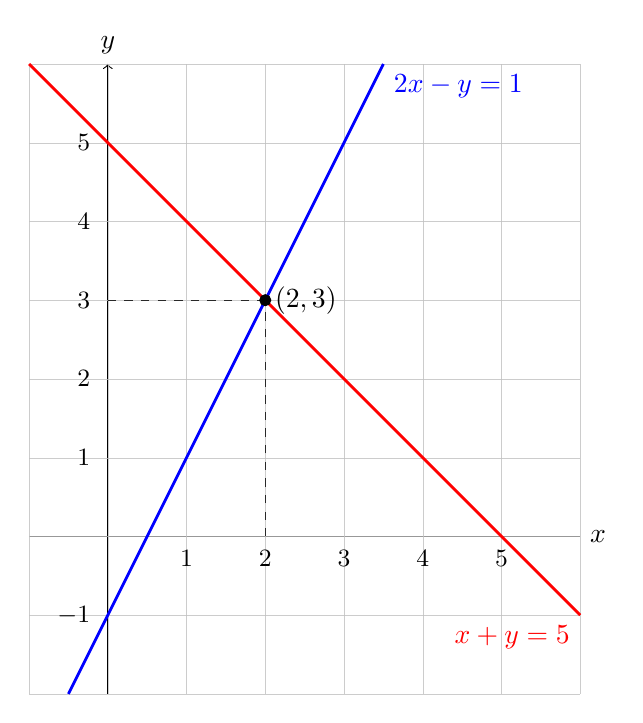
\begin{tikzpicture}
        % Axes:
        \draw[line width=0.4, color=black, arrows=->] (-1, 0) -- (6, 0)
                                                      (0, -2) -- (0, 6);
        
        % Labels:
        \node[anchor=west] at (6, 0) {$x$};
        \node[anchor=south] at (0, 6) {$y$};

        % Grid:
        \foreach \x in {-1, 0, 1, 2, 3, 4, 5, 6}
            \draw[line width=0.1, color=gray!50, opacity=0.8] (\x, -2) -- (\x, 6);
        \foreach \y in {-2, -1, 0, 1, 2, 3, 4, 5, 6}
            \draw[line width=0.1, color=gray!50, opacity=0.8] (-1, \y) -- (6, \y);
        
        % Labels in axes:
        \foreach \x in {1, 2, 3, 4, 5}
            \node[anchor=south] at (\x, -0.5) {\small{$\x$}};
        \foreach \y in {-1, 1, 2, 3, 4, 5}
            \node[anchor=east] at (-0.1, \y) {\small{$\y$}};

        % Functions:
        \draw[line width=1, color=blue] plot[domain=-0.5:3.5] (\x, 2*\x - 1) node[anchor=north west] {$2x - y = 1$};
        \draw[line width=1, color=red] plot[domain=-1:6] (\x, 5 - \x) node[anchor=north east] {$x + y = 5$};

        % Intersection dot at (2,3):
        \draw[line width=0.5mm, color=black, fill=black] (2, 3) circle (0.05);

        % Intersection dot label:
        \node[anchor=west] at (2, 3) {$\left(2, 3\right)$};

        % Intersection grid:
        \draw[line width=0.1, color=black, opacity=0.8, dashed] (0, 3) -- (2, 3);
        \draw[line width=0.1, color=black, opacity=0.8, dashed] (2, 0) -- (2, 3);
    \end{tikzpicture}
    \caption{Gráfica del sistema de ecuaciones lineales (\ref{eq:1.1.1}).}
    \label{fig:1.1.1}
\end{figure}

Ahora bien, existe una equivalencia entre representar un sistema de ecuaciones lineales en forma de gráfica y representarlo en forma de vectores. Para ello, considere el sistema de ecuaciones (\ref{eq:1.1.1}). Puede ser representado como: \begin{align}
    \underbrace{\begin{bmatrix}2 \\ 1\end{bmatrix}}_{\vec{v_1}} x + \underbrace{\begin{bmatrix}-1 \\ 1\end{bmatrix}}_{\vec{v_2}} y &= \underbrace{\begin{bmatrix}1 \\ 5\end{bmatrix}}_{\vec{b}}, \quad x,y \in \mathbb{R}
    \label{eq:1.1.2}
\end{align}

Dónde la gráfica de cada vector es la siguiente:

\begin{figure}[H]
    \centering
    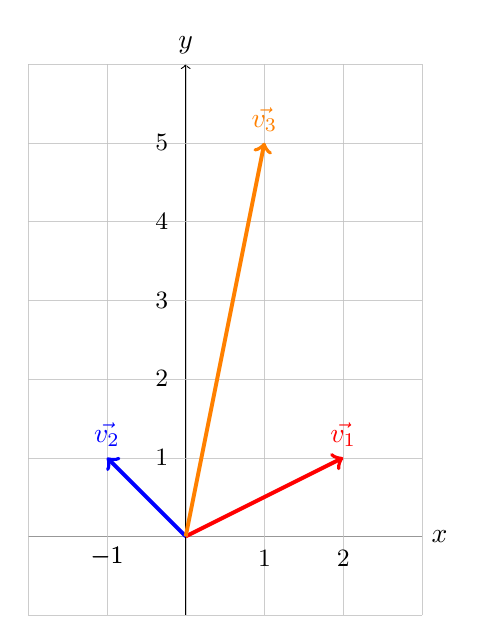
\begin{tikzpicture}
        % Axes:
        \draw[line width=0.4, color=black, arrows=->] (-2, 0) -- (3, 0)
                                                      (0, -1) -- (0, 6);
        
        % Labels:
        \node[anchor=west] at (3, 0) {$x$};
        \node[anchor=south] at (0, 6) {$y$};

        % Grid:
        \foreach \x in {-2, -1, 0, 1, 2, 3}
            \draw[line width=0.1, color=gray!50, opacity=0.8] (\x, -1) -- (\x, 6);
        \foreach \y in {-1, 0, 1, 2, 3, 4, 5, 6}
            \draw[line width=0.1, color=gray!50, opacity=0.8] (-2, \y) -- (3, \y);
        
        % Labels in axes:
        \foreach \x in {-1, -1, 1, 2}
            \node[anchor=south] at (\x, -0.5) {\small{$\x$}};
        \foreach \y in {1, 2, 3, 4, 5}
            \node[anchor=east] at (-0.1, \y) {\small{$\y$}};

        % Dependient vectors
        % \draw[line width=0.5mm, color=gray!80, dashed, opacity=0.5] (0, 0) -- (-3, 3);
        % \draw[line width=0.5mm, color=gray!80, dashed, opacity=0.5] (0, 0) -- (3, 1.5);
        
        % Vectors
        \draw[line width=0.5mm, color=red, arrows=->] (0, 0) -- (2, 1) node[anchor=south] {$\vec{v_1}$};
        \draw[line width=0.5mm, color=blue, arrows=->] (0, 0) -- (-1, 1) node[anchor=south] {$\vec{v_2}$};
        \draw[line width=0.5mm, color=orange, arrows=->] (0, 0) -- (1, 5) node[anchor=south] {$\vec{v_3}$};
    \end{tikzpicture}
    \caption{Óptica vectorial del sistema de ecuaciones (\ref{eq:1.1.1}).}
    \label{fig:1.1.2}
\end{figure}

\subsubsection{Álgebra de vectores}

\begin{enumerate}
    \item \textbf{Producto vectorial:} \begin{align*}
        v_1 \times v_2 = v_1 \times v_2^T &= \underbrace{\begin{pmatrix} \hspace*{0.1cm}\cdot\hspace*{0.1cm} \\ \hspace*{0.1cm}\cdot\hspace*{0.1cm} \end{pmatrix}}_{n\times1} \times \underbrace{\begin{pmatrix} \hspace*{0.1cm}\cdot\hspace*{0.1cm} & \hspace*{0.1cm}\cdot\hspace*{0.1cm} \end{pmatrix}}_{1\times n} = \underbrace{\begin{pmatrix} \hspace*{0.1cm}\cdot\hspace*{0.1cm} & \hspace*{0.1cm}\cdot\hspace*{0.1cm} \\ \hspace*{0.1cm}\cdot\hspace*{0.1cm} & \hspace*{0.1cm}\cdot\hspace*{0.1cm} \end{pmatrix}}_{\text{Matriz } n\times n}
    \end{align*}
    \item \textbf{Producto punto:} \begin{align*}
        v_1 \cdot v_2 &= v_1^T \cdot v_2 = \underbrace{\begin{pmatrix} \hspace*{0.1cm}\cdot\hspace*{0.1cm} & \hspace*{0.1cm}\cdot\hspace*{0.1cm} \end{pmatrix}}_{1\times n} \cdot \underbrace{\begin{pmatrix} \hspace*{0.1cm}\cdot\hspace*{0.1cm} \\ \hspace*{0.1cm}\cdot\hspace*{0.1cm} \end{pmatrix}}_{n\times1} = \underbrace{a}_{\mathbb{R}}
    \end{align*}
    \item \textbf{Producto por un escalar:} \begin{align*}
        \alpha v &= \alpha \begin{pmatrix} v_{11} \\ v_{21} \\ \vdots \\ v_{n1} \end{pmatrix} = \begin{pmatrix} \alpha v_{11} \\ \alpha v_{21} \\ \vdots \\ \alpha v_{n1} \end{pmatrix}
    \end{align*}
\end{enumerate}


\subsubsection{Variable compleja}
\label{sec:1_1}

Sea $z$ una variable compleja, la cual está definida como: \begin{align}
    z = a + ib,
    \label{eq:1.1.3}
\end{align}

dónde, $a$ y $b$ son números reales y $i^2 = -1$.

\paragraph*{Operaciones con números complejos:}

\begin{enumerate}
    \item Suma: \begin{align*}
        z_1 + z_2 &= a_1 + ib_1 + a_2 + ib_2 \\
                    &= (a_1 + a_2) + (ib_1 + ib_2) \\
                    &= (a_1 + a_2) + i(b_1 + b_2)
    \end{align*}
    \item Multiplicación: \begin{align*}
        z_1 z_2 &= (a_1 + ib_1)(a_2 + ib_2) \\
                &= (a_1a_2 - b_1b_2) + i(a_1b_2 + a_2b_1)
    \end{align*}
\end{enumerate}

\subsection{Vectores y matrices}

\begin{definition}[Vector renglón]
{
    \label{def:1.1.1}
    Sea $x$ un vector de $n$ dimensiones, entonces:
    \begin{align*}
        x = (x_1, x_2, \dots, x_n) \in \M_{(1 \times n)}
    \end{align*}
}
\end{definition}

\begin{definition}[Vector columna]
{
    \label{def:1.1.2}
    Sea $x$ un vector de $n$ dimensiones, entonces:
    \begin{align*}
        x = \begin{pmatrix}
            x_1 \\
            x_2 \\
            \vdots \\
            x_n
        \end{pmatrix} \in \M_{(n \times 1)}
    \end{align*}
}
\end{definition}

\begin{definition}[Matriz]
{
    \label{def:1.1.3}
    Sea $A$ una matriz de $m$ renglones y $n$ columnas, está definida como:
    \begin{align*}
        A = \begin{bmatrix}
            a_{11} & a_{12} & \cdots & a_{1n} \\
            a_{21} & a_{22} & \cdots & a_{2n} \\
            \vdots & \vdots & \ddots  & \vdots \\
            a_{m1} & a_{m2} & \cdots & a_{mn}
        \end{bmatrix} \in \M_{(m \times n)}
    \end{align*}
}
\end{definition}

\begin{definition}[Igualdad]
{
    \label{def:1.1.4}
    Sean $A$ y $B$ dos matrices de $m \times n$:
    \begin{align*}
        A = B \quad \Longleftrightarrow \quad \left[a_{ij}\right] = \left[b_{ij}\right], \quad \forall i \forall j
    \end{align*}
}
\end{definition}

\begin{definition}[Suma matricial]
{
    \label{def:1.1.5}
    Sean $A$, $B$ y $C$ matrices de $m \times n$:
    \begin{align*}
        A + B = C \Longleftrightarrow \left[ a_{ij} + b_{ij} \right] = \left[ c_{ij} \right]
    \end{align*}
}
\end{definition}

\begin{definition}[Multiplicación por un escalar]
{
    \label{def:1.1.6}
    Sean $A \in \M_{(m \times n)}$ y $\alpha \in \R$:
    \begin{align*}
        \alpha A = B, \quad B \in \M_{(m \times n)} \quad \Longleftrightarrow \quad \left[ \alpha a_{ij} \right] = \left[ b_{ij} \right]
    \end{align*}
}
\end{definition}

\begin{teorema}
{
    \label{thm:1}
    Sean $A$, $B$ y $C$ matrices de $m \times n$ y $\alpha, \beta$ números reales, entonces: \\

    \begin{enumerate}
        \item $A + \vec{0} = A$
        \item $0A = \vec{0}$
        \item $A + B = B + A$
        \item $(A + B) + C = A + ( B + C )$
        \item $\alpha ( A + B ) = \alpha A + \alpha B$
        \item $1A = A$
        \item $(\alpha + \beta) A = \alpha A + \beta A $
    \end{enumerate}
}
\end{teorema}

\subsection{Producto vectorial y producto matricial}

\begin{align*}
    \text{Sean } a = \begin{pmatrix}
        a_1 \\
        a_2 \\
        \vdots \\
        a_n
    \end{pmatrix}$ y $b = \begin{pmatrix}
        b_1 \\
        b_2 \\
        \vdots \\
        b_n
    \end{pmatrix}
\end{align*}

\begin{definition}[Producto punto]
{
    aaaaaa
}
\end{definition}